\documentclass{article}

\title{Matematica ed Evoluzione}
\author{Sebastian Strozzi}
\date{tratto da: "Un Mondo di Idee"}
\setcounter{secnumdepth}{2}				% non numerare subsubsection

%%%%%%%%%%%%%%%%%%%% Pacchetti %%%%%%%%%%%%%%%%%%%%%						
\usepackage{mathtools}
\usepackage[T1]{fontenc}
\usepackage{lmodern}
\usepackage{textcomp}
\usepackage[utf8]{inputenc}
\usepackage[italian.main, english]{babel}
\usepackage{amsmath}
\usepackage{scalerel}
\usepackage{amssymb}
\usepackage{MnSymbol}
\usepackage{amsthm}
\usepackage{mathrsfs}
\usepackage[shortlabels]{enumitem}
\usepackage[pdfauthor={Sebastian Strozzi},pdftitle={Algebra Lineare e Geometria}]{hyperref}
%	\hypersetup{colorlinks,%
%		citecolor=black,%
%		filecolor=black,%
%		linkcolor=black,%
%		urlcolor=black}
\newcommand\hmmax{0} % default 3
\newcommand\bmmax{0} % default 4
\usepackage{comment} 		            % Usa \begin{comment} \end{comment}
\usepackage{braket} 					% Parentesi
\usepackage{nicefrac}					% Frazioni carine
\usepackage{titlesec}       			% Modifica il formato dei titoli
\usepackage[capitalise]{cleveref} 		% Riferimenti
\usepackage{emptypage} 					% Migliora pagine vuote
%\usepackage{enumitem} 					% Liste
\usepackage{fancyhdr} 					% Modifica stile di pagina

%%%%%%%%%%%%%%%%%% Definizione Comandi %%%%%%%%%%%%%%%%%%%%%%

% Rimuovi la parola 'Chapter' dai titoli
\titleformat{\chapter}
{\Huge \normalfont \bfseries}{\thechapter}{1em}{}


% Stile di Pagina
\pagestyle{fancy}
	\renewcommand{\headrulewidth}{0.1pt}
	\renewcommand{\sectionmark}[1]{%
		\markboth{\thesection.\ #1}{}}
	\lhead{\bfseries \leftmark}
	\chead{}
	\rhead{\bfseries \rightmark}
	\cfoot{\thepage}


% Grafici e Tipografici
\def\barra{\begin{center}	\_\_\_\_\_\_\_\_\_\_\_\_\_\_\_\_\_\_\_\_\_\_\_\_\_\_\_\_\_\_\_\_\_\_\_\_\_\_\_ \end{center}}
\def\Egrave{\MakeUppercase{è}\ }
\def\apertevirg{‘‘}
\def\chiusevirg{''}
\newcommand{\virg}[1]{\apertevirg #1\chiusevirg}

% Insiemi Numerici e Font utili
\def\N{\ensuremath{\mathbb{N}}}
\def\Z{\ensuremath{\mathbb{Z}}}
\def\Q{\ensuremath{\mathbb{Q}}}
\def\R{\ensuremath{\mathbb{R}}}
\def\C{\ensuremath{\mathbb{C}}}
\def\K{\ensuremath{\mathbb{K}}}
\newcommand{\urna}[1]{\ensuremath{\mathbb{#1}}}
\newcommand{\success}[1]{\ensuremath{\underline{#1}}}


% Parentesi
\newcommand{\Graffa}[1]{\ensuremath{ \Big\{ #1 \Big\} }}
\newcommand{\Quadra}[1]{\ensuremath{ \big[ #1 \big] }}

% Simboli Logici e Insiemistici
\def\defeq{\ensuremath{\stackrel{\text{def}}{=}}}				% uguale per def
\def\nn{\ensuremath{\neg}}										% not
\def\ee{\ensuremath{\land}}										% and
\def\oo{\ensuremath{\lor}}										% or
\def\allora{\ensuremath{\Rightarrow}}							% implicazione
\def\sse{\ensuremath{\leftrightarrow}} 							% se e solo se
\def\perogni{\ensuremath{\forall}}								% per ogni
\def\esiste{\ensuremath{\exists}}								% esiste
\def\tc{\ensuremath{\ \rvert\ }}								% tale che
\newcommand{\compl}[1]{\ensuremath{\overline{#1}}}				% complementare
\newcommand{\parti}[1]{\ensuremath{\mathscr{P}(#1)}}			% Parti di X
\def\Universo{\ensuremath{\mathcal{U}}}							% Universo
\def\Partizione{\ensuremath{\mathcal{P}}}						% Partizione
\def\Corr{\ensuremath{\mathcal{C}}}								% Partizione
\def\I{\ensuremath{\mathbb{I}}}									% insieme indice
\def\parallela{\ensuremath{/\!/}}								% simbolo parallele
\newcommand{\class}[1]{\ensuremath{[#1]_{\mathcal{R}}}}			% classe di eq di x


% Simboli Vari
\def\composto{\ensuremath{\circ}}
\def\ts{\ensuremath{\oplus}}
\def\tp{\ensuremath{\otimes}}


% Stile dei Teoremi
\theoremstyle{plain}
\newtheorem{teo}{Teorema}[section]						
\newtheorem{prop}[teo]{Proposizione}
\newtheorem{lemma}[teo]{Lemma}
\newtheorem{corollary}{Corollario}[teo]
\newtheorem{fatto}[teo]{Fatto}
\theoremstyle{definition}
\newtheorem{defin}[teo]{Definizione}
\newtheorem{eg}{Esempio}[chapter]
\newtheorem{es}{Esercizio}[chapter]								

\begin{document}
	\maketitle
	\begin{section}{Modelli Descrittivi} 
		Comprendere un fenomeno reale vuol dire, in fin dei conti, semplificarlo e sottoporne i vari aspetti all’analisi delle scienze descrittive; è da questo atteggiamento che nasce il concetto di modello descrittivo.
		
		\begin{subsection}{Modelli Deterministici}
			
			Quando di un certo sistema si conosce il valore iniziale di un insieme di parametri e si vogliono determinare, in maniera univoca, i valori di quegli stessi parametri a seguito di una certa evoluzione di cui sono note le condizioni, si è davanti ad un modello di tipo deterministico.
			
			Per esempio, se di una freccia conosco la posizione iniziale e le condizioni in cui viene scoccata, un modello deterministico dovrebbe portarmi a conoscere con la desiderata precisione la traiettoria che verrà seguita dalla freccia e, di conseguenza, il punto di arrivo. 
			Chiaramente, più precisione si richiede, migliore dev'essere la conoscenza delle condizioni sotto cui evolve il sistema, ma spesso la natura stessa del problema rende \emph{computazionalmente} impossibile un approccio del genere.
			Anche in biologia, come in fisica, ci sono modelli matematici classici di tipo deterministico per l’interpretazione di alcuni fenomeni, come per esempio il famoso modello di Volterra-Lotka\footnote{Il modello di Volterra-Lotka descrive l’interazione preda-predatore attraverso un sistema di equazioni differenziali non lineari del primo ordine in cui compaiono il numero degli individui per ogni categoria al tempo t, il tasso di crescita e quattro parametri che dipendono dalle particolari specie in esame.}. 
			Per quanto sofisticati, si tratta comunque di modelli analitici che mostrano limiti anche gravi quando vengono applicati a situazioni reali.
				
			Uno dei primissimi problemi che si incontrano nelle analisi di questo tipo è l’enorme quantità di dati che richiede una situazione concreta, intesa come insieme di un enorme numero di fenomeni elementari differenti, per poter essere descritta in modo soddisfacente da un modello deterministico. Questo fenomeno è detto \emph{esplosione combinatoria}.
				
			Consideriamo, per esempio, un modello deterministico che tenti di studiare gli scacchi: nel $1950$ si è stimato che il numero possibile di partite giocabili è, vagamente, $10^{120}$.
			Per capire quanto è grande questo numero, si immagini di costruire un computer in grado di giocare una partita di scacchi differente ogni nanosecondo. Avendo a disposizione tanti computer quanti gli atomi nell'universo e supponendo di farli funzionare tutti contemporaneamente per un tempo uguale all'età dell'universo, non sarebbero sufficienti nemmeno $10'000'000'000'000$ universi per terminatre tutte le possibili partite.
			In altre parole, fissata una certa partita a scacchi, la probabilità di giocare casualmente la stessa partita è circa la stessa che si avrebbe di essere colpiti contemporaneamente da un fulmine e da un meteorite mentre si è su un aereo che sta cadendo esattamente sulla cima del Monte Bianco mentre tutte le centrali nucleari al mondo esplodono contemporaneamente. Da ripetersi tre volte.
			
			Con le opportune modifiche possiamo capire la complessità dei modelli biologici applicati alla realtà: se paragonassimo le mosse degli scacchi, per esempio, con i possibili comportamenti di una specie e l'eito della partita con la sopravvivenza dell'individuo stesso, otterremmo un'idea vaga del perché abbiamo bisogno di idee migliori per studiare questi fenomeni.
			
		\end{subsection}
	
		\begin{subsection}{Modelli Probabilistici}
			
			Un esempio semplice come quello appena discusso fa comprendere la necessità di operare riduzioni drastiche della quantità di dati senza, tuttavia, perdere informazioni essenziali. 
			
			La fisica statistica\footnote{Ad esempio, la Termodinamica con le leggi dei gas perfetti.} utilizza un approccio nel passaggio dalle leggi microscopiche a quelle macroscopiche che offre uno spunto interessante, ma i problemi delle scienze naturali esigono nuovi punti di vista che tengano in considerazione le loro specificità.
			
			Alla matematica si richiede il linguaggio per una formulazione rigorosa ma flessibile di teorie efficaci e di validi modelli che permettano di interpretare i dati osservati e di prevedere l’evoluzione degli aspetti rilevanti di un sistema: nel corso del novecento si sono affermati, accanto ai modelli deterministici classici, i modelli probabilistici. 
			La peculiarità di questi ultimi sta nel riuscire a generalizzare grandi classi di problemi senza rinunciare alla specificità di ognuno di essi, risultando così di grande utilità pratica anche in biologia per via delle enormi capacità descrittive e predittive unite ad un netto alleggerimento computazionale.
			
			Negli ultimi decenni l’affermazione della biologia molecolare ha sollecitato poi l’uso di strumenti matematici del tutto diversi. Oltre all’imposizione di un’analisi probabilistica di molti fenomeni biologico-molecolari, la natura stessa dei problemi trattati ha dato agli oggetti matematici in esame un carattere discreto e un contenuto combinatorico e algebrico. 
			Questo ha richiesto l’uso e, in alcuni casi, la creazione di raffinate tecniche algebrico-geometriche. Si tratta dunque di un quadro completamente nuovo ed estremamente stimolante sia per i matematici che per i biologi.
		\end{subsection}
	\end{section}
	\newpage
	
	\begin{section}{Modelli per la Biologia Molecolare}

		\begin{subsection}{Biologia Molecolare}
			
			\begin{center} \emph{(Disclaimer: it's not my cup of tea)} \end{center}
			La biochimica, nata dalla fisiologia nei primi anni del Novecento, studia in maniera approfondita le proprietà e le funzioni delle molecole che compongono la materia vivente.
		
			Gregor Mendel, padre della genetica, postulò l’esistenza di unità discrete di informazione, i geni, che governano la trasmissione delle caratteristiche individuali in un organismo. 
			Nella prima metà del Novecento si capì che i geni sono contenuti nelle macromolecole complesse di acido desossiribonucleico e nel 1953 Watson e Crick determinarono la struttura del DNA: una catena di molecole più semplici organizzate in due catene avvolte a spirale a formare una doppia elica. 
			L’informazione genetica contenuta nel DNA è codificata in una successione di basi azotate: adenina A, timina T, citosina C e guanina G. 
			Le basi azotate di un’elica determinano quelle dell’altra. Infatti ogni base su una catena è legata a una base complementare sull’altra. Le coppie complementari sono (C, G) e (T, A). Una determinata sequenza di coppie di basi azotate costituisce un gene; l'informazione viene interpretata secondo una corrispondenza tra basi azotate e amminoacidi. In tal modo i geni regolano la sintesi delle proteine. 
			
			Dal punto di vista genetico ogni specie viene descritta dal suo DNA, la cui struttura primaria si modella come una stringa, cioè una sequenza di lettere, sull’alfabeto: $$ \Omega = \{ A, C, G, T \}$$
			Il contenuto totale delle molecole di DNA costituisce il genoma di un organismo. Il genoma umano, formato da circa 3 miliardi di coppie di basi complementari, corrisponde a circa 700 MB di informazione. 
			Il genoma di due individui della stessa specie non è identico: le differenze per gli esseri umani sono di circa una base ogni mille, sufficienti però a spiegare la variabilità tra i diversi individui. 
			
			La successione delle basi in un segmento di DNA e quella degli amminoacidi in una proteina sono esempi di sequenze biologiche. Basilari problemi in biologia molecolare sono il riconoscimento e l’estrazione dell’informazione codificata in una sequenza biologica. Per esempio è importante:
			\begin{enumerate}[1)]
				\item distinguere la parte di un gene che codifica una proteina dalla parte non codificante;
				\item segmentare una porzione di DNA in frazioni con diverse funzioni;
				\item allineare porzioni di DNA appartenenti a specie diverse, allo scopo di determinare una distanza biologicamente significativa fra le specie;
				\item costruire un albero filogenetico.
			\end{enumerate}
		\end{subsection}
	%\newpage
		\begin{subsection}{Modelli Probabilistici per la Biologia Molecolare}
			
			Supponiamo di osservare, per la descrizione di sequenze biologiche, una successione di lettere del nostro alfabeto $\Omega$.
			Vogliamo costruire un modello probabilistico che ci consenta di generare questi dati, ma considerare una semplice estrazione casuale da un’urna contenete un certo numero di A, C, G e T risulterebbe troppo semplicistico in quanto presupporrebbe l’indipendenza tra caratteri, che non è biologicamente plausibile. Infatti, parlando di codoni, più triplette possono codificare per una stessa proteina. Queste triplette differiscono le une dalle altre solo per l’ultima base: in altre parole, le basi azotate che appaiono nella terza posizione di ogni codone hanno una probabilità di cambiare significativamente maggiore delle altre in quanto producono modificazioni sinonime.
			
			\begin{subsubsection}{Catene di Markov}
				Abbiamo quindi bisogno di un modello che tenga conto di questa dipendenza: consideriamo quattro urne, la prima marcata con \urna{A}, la seconda con \urna{C}, la terza con \urna{G}, la quarta con \urna{T} e una quinta marcata con \urna{I} (per \virg{inizializzazione}).
				Nell’urna \urna{A} ci sono $n_{\urna{A},A}$ palline marcate con A, $n_{\urna{A},C}$ marcate con C ecc... 
				In generale, l’urna \urna{X} contiene $n_{\urna{X},Y}$ palline contrassegnate con Y$\in \Omega$.
				Infine, l’urna \urna{I} contiene $n_A$ palline marcate con A, $n_C$ palline marcate con C e così via.
				
				Il processo di generazione di una sequenza consiste nei passi seguenti:
				\begin{enumerate}[1)]
					\item \textbf{Inizializzazione}: estrarre una pallina dall’urna \urna{I};
					\item \textbf{Iterazione}: estrarre una pallina dall’urna contrassegnata dalla lettera scritta sulla pallina pescata al passo precedente (i.e. la pallina marcata con A manda all'urna \urna{A}), annotare la lettera, rimettere la pallina nell’urna e mescolare;
					\item ripetere il passo di iterazione.
				\end{enumerate}
				Questo modello così costruito garantisce un meccanismo di dipendenza nella generazione della sequenza, infatti l’estrazione di una certa lettera dipende da quella estratta al passo precedente (e soltanto da quella).
				La dipendenza è chiarita dai valori delle probabilità delle varie estrazioni che sono $p_A$, $p_C$, $p_G$ e $p_T$ per l’urna I ed invece: $$ p_{\urna{X},Y} = \frac{n_{\urna{X},Y}}{n_{\urna{X},A}+n_{\urna{X},C}+n_{\urna{X},G}+n_{\urna{X},T}} $$ la probabilità di pescare una pallina marcata con Y$\in \Omega$ dall’urna \urna{X}.
				
				\Egrave evidente che la probabilità di estrarre una pallina Y cambia a seconda dell'urna in cui mi trovo: pescare una pallina K o una pallina J al passo $n$-esimo può cambiare anche significativamente la probabilità di pescare Y al passo successivo (K,J,Y$\in \Omega$).
				
				I parametri di questo modello sono quindi le probabilità di estrazione di ogni urna. Sarà necessario caprie come stimare questi parametri al fine di avere un modello adeguato.
			\end{subsubsection}
		
			\begin{subsubsection}{Modelli a stati nascosti}
				Nella realtà ci sono, tuttavia, dati che sfuggono alla possibilità di osservazione: l’esito (osservabile) di una verifica dipenderà verosimilmente dall'agitazione (non osservabile) avvertita dall'alunno. 
				C’è quindi l’esigenza di introdurre altre variabili nel modello probabilistico che prenderanno il nome di \virg{stati nascosti}, cioè stati non osservabili che però influenzano le osservazioni.
				
				Un semplice modello a stati nascosti può essere costruito considerando due urne chiamate “Testa” e “Croce”, ciascuna contenente palline marcate A, C, G, T e una moneta con due facce distinguibili ma non necessariamente equiprobabili, ognuna delle quali conduce ad una delle due urne. Come prima $p_{\urna{X},Y}$ di estrarre la pallina marcata con Y dall’urna \urna{X} è funzione dei numeri $n_{\urna{Z},Y}$ di palline marcate Y nell’urna \urna{Z}. 
				Una sequenza sarà quindi generata così: 
				\begin{enumerate}[1)]
					\item si lancia la moneta;
					\item si pesca una pallina dalla corrispondente urna annotandone la lettera;
					\item si rimette la pallina nell’urna e si rimescola, quindi si ripete.
				\end{enumerate}
				Questo modello descrive un processo visibile, quello delle estrazioni che producono la sequenza, basato però su un processo non osservabile, il lancio della moneta. 
				Anche in questo caso però non è un modello adeguato alla descrizione di sequenze biologiche: non è realistico supporre che gli eventi del processo nascosto siano indipendenti come il lancio di una moneta.
			\end{subsubsection}
			
			\begin{subsubsection}{Catene di Markov a stati nascosti}
				Per introdurre una forma di dipendenza tra gli stati nascosti possiamo modellarli come una catena di Markov: consideriamo per esempio due tavoli contrassegnati da “Testa” e “Croce”; su ogni tavolo poniamo un’urna come quella descritta nel generico modello a stati nascosti, contrassegnata con lo stesso simbolo del tavolo ed una moneta con facce distinguibili e, anche in questo caso, non necessariamente equiprobabili. Le due monete possono essere truccate differentemente a seconda delle osservazioni raccolte. Consideriamo infine una terza moneta come le due appena descritte per inizializzare il processo.
				
				Il processo di generazione di una sequenza consiste adesso nei passi seguenti:
				\begin{enumerate}[1)]
					\item \textbf{Inizializzazione}: si lancia la terza moneta per scegliere il tavolo da cui cominciare;
					\item \textbf{Iterazione}: si pesca una pallina dal tavolo corrente, si annota la lettera che la contrassegna reinserendola poi nell’urna, quindi si lancia la moneta del tavolo corrente per scegliere il nuovo tavolo;
					\item si ripete il passo di iterazione.
				\end{enumerate}
				Questo processo costituisce un essenziale modello per descrivere alcuni aspetti delle sequenze biologiche.
			\end{subsubsection}
			
			\begin{subsubsection}{Generalizzazione ed Analisi(*)}
				Possiamo ulteriormente generalizzare la nostra catena di Markov a stati nascosti coi seguenti dati:
				\begin{enumerate}[1.]
					\item L’alfabeto $N = \{n_1, \ldots, n_m\}$ degli stati nascosti;
					\item L’alfabeto $V = \{v_1, \ldots, v_k\}$ dei simboli visibili;
					\item Il vettore $p = \{p_1, \ldots, p_m\}$ delle probabilità\footnote{La componente $i$-esima $p_i$ è la probabilità che lo stato iniziale sia $n_i$} iniziali;
					\item La matrice $T = (t_{ij})$ di transizione\footnote{$t_{ij}$ è la probabilità di passare dallo stato $n_i$ allo stato $n_j$} tra gli stati nascosti ($1\leq i,j\leq m$);
					\item La matrice $E = (e_{is})$ di emissione\footnote{$e_{is}$ è la probabilità che lo stato $n_i$ emetta il simbolo $v_s$} ($1\leq j\leq m$ e $1\leq s \leq k$).
				\end{enumerate}
				Il vettore $p$ chiarisce com'è truccata l’estrazione iniziale di uno dei tavoli (stato nascosto), scelti nell’insieme $N$, da cui poi verrà estratto il primo simbolo visibile della sequenza. 
				La matrice $E$ di emissione contiene le informazioni sulle probabilità di pescare un certo simbolo dall’urna situata sul tavolo in cui ci troviamo. 
				Per passare da un tavolo al successivo lanciamo la moneta di $m$ facce associata al tavolo attuale e truccata secondo quanto riportato nella matrice $T$ di transizione, quindi estraiamo un nuovo simbolo visibile e, dopo averlo annotato, cambiamo nuovamente tavolo fino alla conclusione del processo.
				
				\begin{center}
					\vspace{15pt}
					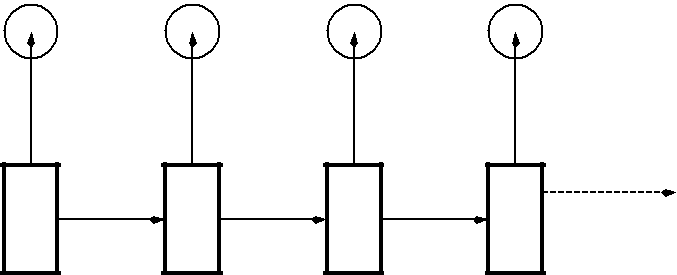
\includegraphics[width=0.5\textwidth]{Pics/markov.png}
					\\ \vspace{6pt}
					\emph{Diagramma associato al processo appena descritto: \\ le frecce verso l’alto rappresentano l’emissione, \\ mentre quelle verso destra la transizione.}
					\vspace{12pt}
				\end{center}
				Consideriamo ora una successione fissata di stati nascosti: $$ \success{m} = (m_1, \ldots, m_n) \quad m_i\in N $$ e denotiamo con $\aleph$ l’insieme di tutte le possibili sequenze $m$. Consideriamo poi una successione di stati visibili: $$ \success{s} = (s_1, \ldots, s_n) \quad s_i \in V $$
				La probabilità di trovare la sequenza $s$ in corrispondenza degli stati nascosti $m$ è: $$ p_{\success{ms}} = p_{m_1}e_{m_1s_1}t_{m_1m_2}e_{m_2s_2}t_{m_2m_3}e_{m_3s_3}\cdots t_{m_{n-1}m_n}e_{m_ns_n} $$ che è un monomio le cui lettere sono i parametri del nostro modello. 
				
				Possiamo quindi scrivere la probabilità di osservare $\success{s}$ al variare dei parametri nascosti $\success{m}$ ed otterremo il polinomio: $$ p_{\success{s}} = \sum_{n\in\aleph}^{}p_{\success{ms}} $$ 
				
				Il polinomio ottenuto sarà ciò che ci permetterà di determinare1 i parametri del modello e, allo stesso tempo, darà anche luogo a sofisticati metodi di verifica dell’adeguatezza dello stesso. Basta inoltre considerare che l’alfabeto $V$ degli stati visibili sia uguale ad $\Omega$ ($V=\Omega$) per ottenere una descrizione biologica caratterizzata da una grandissima flessibilità.
			\end{subsubsection}
			
		\end{subsection}

	\end{section}
	\newpage

	\begin{section}{Metodi Matematici per la Filogenetica}
		\begin{quote}
			| \textit{«L'ontogenesi è una ricapitolazione della filogenesi.»}
		\end{quote}
		Sebbene l'ipotesi originale, espressa nella citazione, sia stata rigettata perché troppo superficiale, la biologia moderna riconosce molteplici connessioni fra ontogenia e filogenia, spiegandole attraverso la teoria dell'evoluzione e considerandole come argomenti in suo favore.
		A parte il suo interesse teorico, che consiste nel capire come si sviluppano i meccanismi evolutivi delle specie, la filogenetica gode di importanti applicazioni pratiche tra cui: capire l’evoluzione di differenti ceppi virali allo scopo di determinarne la pericolosità e capire la possibilità di trovare vaccini efficaci (\emph{utile, eh?}); o, ancora, stimare la distanza evolutiva tra diverse specie al fine di estendere l’efficacia di interventi terapeutici come trapianti o somministrazione di farmaci.
		
		\begin{subsubsection}{Il Problema Fondamentale}
			La teoria evoluzionistica di Darwin presuppone che le specie si evolvano da antenati comuni, quindi prevede l’esistenza di strutture, detti \emph{alberi filogenetici}, alla cui radice vi è l’antenato comune delle specie che si trovano alle foglie. 
			Gli alberi filogenetici mostrano dunque le relazioni evolutive tra diverse specie o altre entità biologiche che si suppone abbiano un antenato comune. 
			
			Il problema fondamentale della filogenetica è il seguente: date delle specie e delle osservazioni a esse relative, si vuole determinare l’albero filogenetico che è in migliore accordo con le osservazioni sulla base di una serie di ipotesi di lavoro. 
			
			La costruzione degli alberi filogenetici è, in generale, un problema insolubile per la sua enorme complessità. Nella pratica, però, è possibile determinare alberi filogenetici che descrivono solo alcuni aspetti evolutivi di un ristretto insieme di specie, sfruttando un numero limitato di caratteri, che possono essere morfologici oppure biochimici.
			
			La filogenesi molecolare utilizza le informazioni sulle differenze delle strutture molecolari di DNA, RNA e proteine, per costruire un albero filogenetico che indica la probabile evoluzione dei vari organismi. 
			A seguito del processo evolutivo, anche il DNA subisce delle corrispondenti modifiche, che sono tanto più marcate, quanto più \emph{lontane} sono le specie evolutesi nel tempo. 
			Pertanto, organismi strettamente connessi hanno generalmente un alto grado di accordo nella struttura molecolare del DNA (e quindi delle sostanze ad esso legate quali RNA e proteine), che però mostra delle marcate differenze in organismi remotamente connessi.
		\end{subsubsection}
	
		\begin{subsection}{Teoria dei Grafi e degli Alberi}
			La nozione di albero filogenetico non è altro che un caso particolare della ben nota nozione di \emph{grafo}, utilizzata in matematica, informatica e numerosi altri contesti scientifici per dare una forma tangibile alle relazioni tra coppie di elementi di un insieme.
			
			Il primo a cogliere l’importanza del concetto di grafo è stato Leonhard Euler. Il problema di cui si occupò Eulero è il cosiddetto \emph{problema dei ponti di Könisberg}: nella città di Könisberg ci sono due grosse isole nel fiume Pregel, collegate tra loro e con il resto della città da 7 ponti. Il problema consiste nel trovare, se possibile, un percorso che attraversi tutti ponti esattamente una volta e riporti al punto di partenza.
			Eulero rappresentò ognuna delle quattro zone in cui il fiume divide la città con un \emph{nodo} ed ogni ponte che congiunge due zone con un \emph{arco} tra i corrispondenti nodi, cioè attraverso il multigrafo:
			\begin{center}
				\vspace{9pt}
				\hfill
				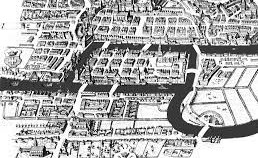
\includegraphics[height=60pt]{Pics/konisberg.png} \hfill
				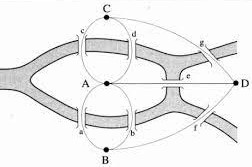
\includegraphics[height=60pt]{Pics/konisberg1.png} \hfill
				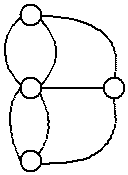
\includegraphics[height=60pt]{Pics/multigrafo1.png}
				\hfill
				\vspace{9pt}
			\end{center}
		
			Eulero capì che la risolubilità del problema dipende dal numero degli archi che escono da ciascun nodo: dimostrò che un percorso della forma desiderata esiste \emph{se e solo se} tutti i nodi vedono un numero pari di archi. Queste premesse permisero lo sviluppo di una teoria del tutto nuova.
			
			Innanzitutto, un grafo $(V,A)$ è dato da un insieme finito $V$ di punti, detti \emph{vertici}, e un insieme finito $A$ di \emph{archi}, ognuno dei quali connette una coppia di vertici non necessariamente distinti, che si dicono \emph{adiacenti}.
			
			Dal grafo rappresentato sopra si nota che è possibile avere più archi che connettono una stessa coppia di vertici. Si dice \emph{grado} di un vertice il numero degli archi che lo contengono. 
			
			\Egrave possibile rappresentare un grafo con un diagramma, disegnando per ogni vertice un pallino e congiungendo con delle linee i pallini che rappresentano vertici adiacenti. Osserviamo che diagrammi diversi possono rappresentare lo stesso grafo, come nelle seguenti figure:
			\begin{center}
				\vspace{6pt}
				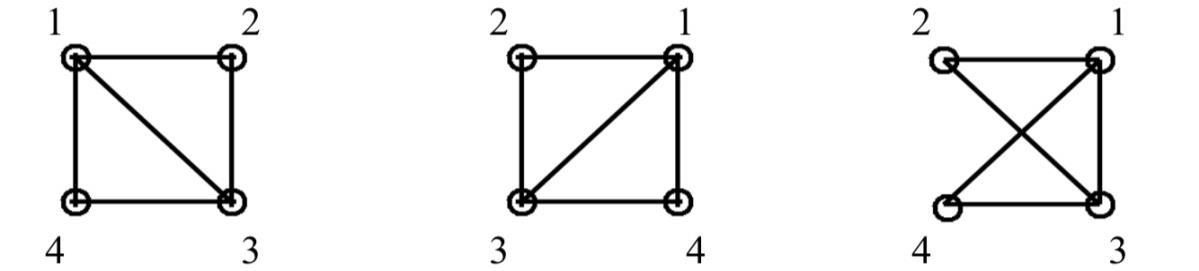
\includegraphics[width=0.7\textwidth]{Pics/diagramma1.png}
				\vspace{6pt}
			\end{center}
		
			Tuttavia, due grafi possono essere diversi soltanto per i nomi che si sono dati ai vertici: in tal caso si dicono \emph{isomorfi} e hanno le stesse proprietà. 
			Consideriamo, da qui in poi, grafi in cui ogni coppia di vertici è collegata da al più un arco e non vi sono archi che collegano un vertice a se stesso.
			Definiamo \emph{cammino} una successione di vertici adiacenti $\{V_1, V_2, \ldots, V_n\}$, in altre parole, è un percorso che permette di andare da $V_1$ a $V_n$ passando per i vertici \virg{intermedi} attraverso gli archi del grafo. Se $V_1 = V_n$ allora il cammino si dice \emph{chiuso} e, se $\perogni i,j \neq n$ distinti $\allora V_i \neq V_j$, il cammino si dice \emph{ciclo}. 
			Di contro, un grafo senza cicli si dice \emph{aciclico}. 
			
			Se comunque scelti due vertici del grafo esiste almeno un cammino tale da averli come estremi, il grafo si dice \emph{connesso}.
			
			Un \emph{albero} è definito come un grafo connesso e aciclico nel quale gli archi sono chiamati anche \emph{rami}. Chiamiamo \emph{foglia} di un albero ogni vertice di grado 1. Un albero si dice \emph{binario} se ha al più un vertice di grado 2, che si dice radice, e ogni altro vertice che non sia una foglia ha grado 3. 
				\begin{center}
					\vspace{6pt}
					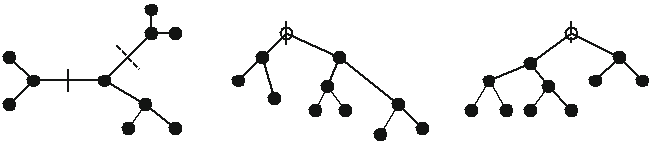
\includegraphics[width=0.6\textwidth]{Pics/rooted1.png}
					\\ \vspace{6pt}
					\emph{In figura è rappresentato un albero binario senza radice \\ e due dei molti modi per aggiungergli una radice.}
					\vspace{6pt}
				\end{center}
			
			Per descrivere l’evoluzione delle specie biologiche si utilizza la struttura di \emph{albero filogenetico} o \emph{filogenia}: si tratta di un albero binario le cui foglie sono \emph{etichettate}, ossia un albero binario in cui ad ogni foglia è assegnato un nome. Nella pratica, ogni foglia rappresenta una specie osservata ed è importante sottolineare che un isomorfismo tra alberi etichettati deve anche preservare le etichette, dunque non tutti gli alberi isomorfi sono isomorfi anche come alberi etichettati. 
			
			L’idea di isomorfismo riveste un ruolo cruciale nell’analisi scientifica: due alberi sono isomorfi se è possibile ottenere il primo \virg{ripiegando} il secondo, ciò vuol dire che, a meno di un fattore quasi meramente estetico, i due alberi in questione non sono altro che due facce della stessa medaglia o, in altre parole, due modi di esprimere lo stesso concetto: di ogni classe di isomorfismo di grafi posso quindi scegliere solo un rappresentante e trascurare, nei calcoli, tutti gli altri. 
			
			Il numero degli alberi binari con radice e $k$ foglie etichettate non isomorfi è tuttavia enorme già per valori piccoli di $k$, esso è infatti $(2k-3)!!$\footnote{$(2k-3)!!$ indica il semifattoriale di $2k-3$, cioè il prodotto di un numero dispari per tutti i dispari a lui precedenti o di un numero pari per tutti gli altri pari più piccoli di lui. È facile intuire che 2k-3 è sempre dispari, quindi ricadiamo nel primo caso.} e questo rende impossibile l’elencazione, ai fini valutativi, di tutte le possibili filogenie quando il numero di specie ($=k$) è superiore a qualche decina. In altre parole, è inattuabile l'approccio \emph{naïf} di elencare ogni possibile albero e scegliere \virg{a mano} quello migliore.
		\end{subsection}
		
		\begin{subsection}{Inferenza dell’Albero Filogenetico dai dati}
			La determinazione dell’albero filogenetico migliore per una certa sequenza di dati osservati è un procedimento spesso complicato e laborioso.
			Consideriamo, per semplicità, tre caratteri dicotomici, cioè che possono acquisire soltanto due valori, e tre diverse specie. Costruiamo la seguente matrice:
			\begin{align*}
				 a \quad   b \quad   c \quad \; \\
				\begin{array}{c}
					c_1 \\ c_2 \\ c_3
				\end{array}
				\left(
				\begin{array}{ccc}
					1 & 1 & 0 \\
					0 & 0 & 1 \\
					1 & 0 & 1
				\end{array} \right)
			\end{align*}
			dove le specie sono indicate con le lettere $a$, $b$ e $c$ mentre i caratteri con $c_1$, $c_2$ e $c_3$. 
			Un carattere dicotomico, come quelli che stiamo considerando in questo esempio, si può interpretare come presenza/assenza di una certa qualità (i.e. avere o no gli occhi azzurri). In particolare, la specie $a$ possiede i caratteri $c_1$ e $c_3$ ma non $c_2$.
			
			Si noti che quanto detto si applica anche nel caso in cui la caratterizzazione sia fatta allineando tratti di DNA di diverse specie: in questo caso la matrice dei dati conterrà le sequenze biologiche osservate per una data specie. In altre parole, invece di $0$ e $1$ avremo le lettere $A$, $C$, $G$ e $T$, mentre i \virg{caratteri} saranno la posizione nella catena di DNA.
			
			Tornando al nostro esempio, esistono tre diversi alberi filogenetici, a meno di isomorfismi, che abbiano le tre specie $a$, $b$ e $c$ alle foglie:
			\begin{center}
			% 	\vspace{3pt}
				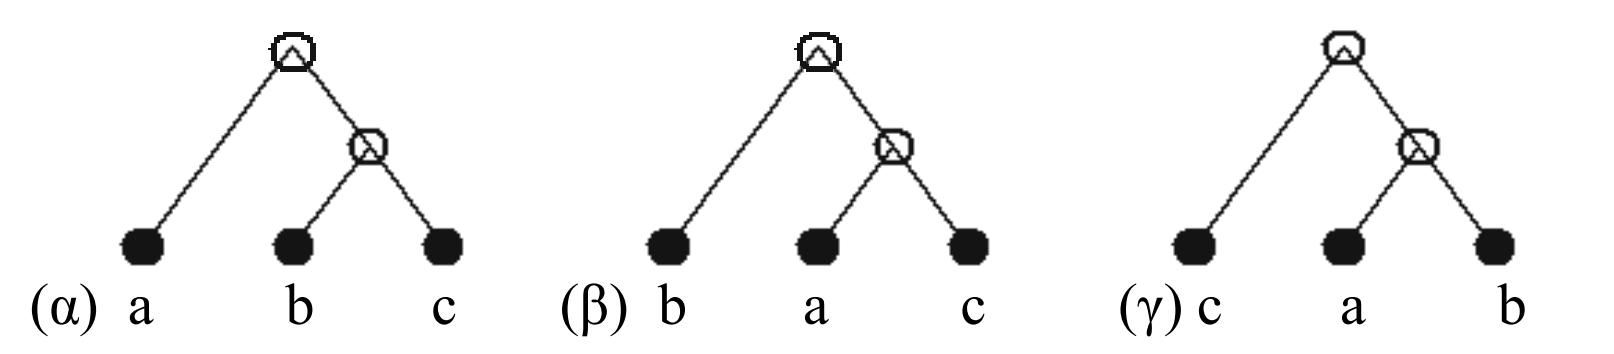
\includegraphics[width=0.6\textwidth]{Pics/alberi1.png}
			%	\\ \vspace{3pt}
			\end{center}
			Dobbiamo decidere quale di questi sia il migliore in accordo con la matrice dei dati osservati.
			\begin{subsubsection}{Metodo diretto}
				In questo semplice caso l’albero più adatto è $\gamma$ in virtù di una facile osservazione: i primi due caratteri ($c_1$ e $c_2$) accomunano $a$ e $b$, infatti assumono per entrambi lo stesso valore, per $c$ assumono invece un valore differente; un solo carattere accomuna $a$ con $c$, distinguendo entrambi da $b$. 
				
				Poniamo quindi più vicine le due specie che hanno più caratteri in comune, lasciando $c$ distante; la scelta della posizione $c-a-b$ oppure $c-b-a$ è ininfluente in quanto darebbe luogo a due alberi etichettati isomorfi tra loro. \Egrave chiaro che questo approccio diretto non è utilizzabile in situazioni più complicate.
			\end{subsubsection}
		
			\begin{subsubsection}{Metodo di Massima Parsimonia}
				Secondo questo metodo si giudicano più plausibili gli alberi che spiegano i caratteri delle foglie con il minimo numero totale di cambiamenti a partire dalla radice.
				Per ogni albero possiamo \virg{scegliere} un antenato da porre alla radice (i.e. fissare arbitrariamente un valore per ogni carattere). 
				Percorrendo i diversi rami dell’albero, ogni valore scelto per la radice potrebbe andare incontro a dei cambiamenti lungo l’arco per ottenere i valori dell’individuo alla foglia verso cui si è andati. Fissato un certo antenato, qual è il numero minimo di cambiamenti necessari per ottenere, alle foglie, i valori osservati? E la scelta dell'antenato è influente?
				Riprendendo l'esempio iniziale, consideriamo l’albero $\alpha$ ed il solo carattere $c_1$: sceglialo per lo stato di $c_1$ alla radice il valore $0$, sono quindi necessari almeno due cambiamenti per ottenere i valori osservati di $c_1$ alle foglie, infatti:
				\begin{center}
					\vspace{3pt}
					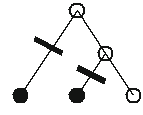
\includegraphics[width=0.25\textwidth]{Pics/parsimonia.png}
					\\ \ \, \textbf{a} \qquad \ \, \textbf{b} \ \qquad\, \textbf{c}
					\\ \vspace{6pt}
					\emph{Il segmento in grassetto nella figura indica un cambiamento, \\ mentre lo stato del carattere viene indicato dal colore \\ della pallina: bianco per zero e nero per uno.}
					\vspace{6pt}
				\end{center}
				
				Scegliendo come valori per i tre caratteri alla radice $(0, 1, 0)$ si può verificare che, nel complesso, il numero minimo di cambiamenti necessari per ottenere i valori osservati alle foglie è $6$. Se invece si scelgono i valori $(1, 0, 1)$ per l'antenato alla radice, allora il numero minimo di cambiamenti è $3$, che è anche il più piccolo numero di cambiamenti possibili per questo albero. Effettivamente, nel singolo albero, il numero di cambiamenti varia al variare della scelta dell'antenato. Tuttavia i singoli caratteri non si influenzano a vicenda, quindi ottimizzare il numero totale di cambiamenti equivale ad ottimizzare il numero di cambiamenti per ogni singolo carattere. In ogni caso si cerca il numero minimo \emph{al variare dell'antemato}: in pratica gli antenati che minimizzano il numero del singolo alero potrebbero essere differenti, ma a prescindere dall'antenato, un albero sarà preferibile ad un altro se il numero minimo del primo è minore del numero minimo del secondo.
				
				L'esempio di prima, tuttavia, è \emph{ad hoc} per mostrare i limiti di questo metodo: anche per $\beta$ e $\gamma$ il numero minimo di cambiamenti è $3$, corrispondenti rispettivamente alle scelte $(1, 0, 1)$ e $(1, 1, 1)$ degli antenati alla radice. Nel nostro esempio non è quindi possibile scegliere quale sia l’albero più adatto usando il principio di massima parsimonia, eppure per confronto diretto sappiamo che un albero migliore effettivamente \emph{esiste}.
				
				In generale, in effetti, tale principio è in grado di determinare, se non un unico albero \virg{parsimonioso}, almeno un piccolo insieme\footnote{Una riduzione del genere potrebbe essere di grande utilità in quanto permetterebbe di restringere parecchio lo spazio delle possibilità. E, sognando un po', potrebbe addirittura rendere sensato il metodo diretto. Tuttavia, spesso, i risultati non sono tali da ripagare lo sforzo computazionale.} di alberi ugualmente validi tra tutti i possibili. Tra quelli ottenuti, poi, si potrà eventualmente applicare un metodo differente. \par
				
				A titolo esemplificativo, si considerino $5$ specie e, per ognuna, si osservino $6$ caratteri binari secondo la matrice:
				
				\begin{align*}
					\begin{array}{c|ccccc}
						\phantom a & S_1 & S_2 & S_3 & S_4 & S_5 \\ \hline
						c_1 & 1 & 0 & 1 & 1 & 0 \\ 
						c_2 & 0 & 0 & 1 & 1 & 0 \\
						c_3 & 0 & 0 & 1 & 1 & 0 \\
						c_4 & 0 & 0 & 1 & 1 & 0 \\
						c_5 & 1 & 0 & 1 & 0 & 0
					\end{array}
				\end{align*}	
				\vspace{6pt} \\
				L’albero di massima parsimonia è:
				\begin{center}
					\vspace{6pt}
					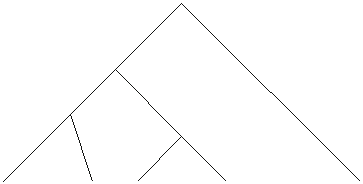
\includegraphics[width=0.4\textwidth]{Pics/parsimonia2.png}
					\\
					\emph{$\ \; \mathbf{S_4} \qquad \; \mathbf{S_3} \quad \mathbf{S_2} \qquad \mathbf{S_5} \qquad \qquad \mathbf{S_1}$}
					\vspace{9pt}
				\end{center}
				per il quale sono sufficienti $8$ cambiamenti per ottenere le osservazioni.
				
				Esistono anche, in effetti, algoritmi efficaci, di tipo combinatorico, per contare il numero minimo di cambiamenti necessari a ottenere i dati osservati per un certo albero. Tuttavia, per quanto concettualmente semplice, la determinazione di un albero filogenetico secondo il principio di massima parsimonia comporta un grande costo computazionale. È necessario, infatti, considerare uno ad uno tutti gli alberi filogenetici aventi un dato numero di etichette e, come abbiamo visto, questo numero cresce enormemente al crescere delle specie osservate.
				
				In sostanza, si tratta di un metodo che rimpiazza l'osservazione \virg{umana} nel metodo diretto, ma non c’è speranza di usarlo, proprio come il metodo diretto, per determinare le filogenie quando il numero di specie supera la decina. 
				Esistono comunque algoritmi efficaci per la ricerca di buone approssimazioni della soluzione ottimale: essi evitano di considerare tutte le filogenie con un dato numero di foglie. Per fare ciò, usano una struttura matematica più raffinata che \virg{parla} dell’intero insieme degli alberi filogenetici con un dato numero di foglie invece che di ciascuno singolarmente. 
				
				Ironicamente, anche l’insieme degli alberi filogenetici con un dato numero di foglie ha, a sua volta, struttura di grafo. \Egrave detto \emph{grafo degli alberi filogenetici} e, in esso, ogni albero filogenetico assume a sua volta il ruolo di vertice evidenziando così le coppie di alberi adiacenti.
				
				Partendo da un albero filogenetico qualsiasi in questo grafo, si \virg{visitano} tutti quelli adiacenti e, tra questi, si sceglie il migliore. Da questo si ricomincia. 
				Di contro, quello che si ottiene è un \emph{ottimo locale}: è evidente che esso non ha alberi adiacnti migliori di esso, né ve ne sono sull'intero cammino percorso, ma nessuno ci garantisce che sia migliore anche di quelli che non sono stati visitati. In effetti, un ottimo locale può comunque essere ben lontano dall’essere anche solo una buona soluzione al problema che ci siamo posti. 
				
				Esistono espedienti, di carattere probabilistico, volti ad evitare di rimanere \virg{intrappolati} in un ottimo locale non soddisfacente. In breve, si esplora il grafo degli alberi filogenetici con una \emph{passeggiata aleatoria}. Essa, in effetti, ammette che con una certa probabilità si possa compiere una transizione a uno stato sfavorito, ma questa transizione è tanto più improbabile quanto peggiore è il nuovo stato rispetto a quello iniziale. Oltretutto, si chiede che questo meccanismo di transizione agli stati sfavoriti diventi sempre meno probabile con l’aumentare della durata della passeggiata\footnote{Si può visualizzare questo procedimento come il viaggio di un esploratore su di un suolo montuoso alla ricerca della zona a quota più bassa possibile: l’esploratore tenderà sempre a scendere verso la valle in cui si trova, ma deciderà di controllare le vallate circostanti solo a patto che le montagne che la separano da quella attuale non siano troppo alte e che la stanchezza non sia tale da impedirgli di proseguire.}. Questo per assicurarsi che, prima o poi, il processo termini.
			\end{subsubsection}
		
			\begin{subsubsection}{Metodo di Massima Verosimiglianza}
				Per applicare questo metodo, bisogna capire come associare una probabilità a delle osservazioni generiche. Tale assegnazione richiede quindi un modello probabilistico in grado di generare le osservazioni.
				
				Partiamo da un esempio elementare. Consideriamo una sequenza assegnata, di lunghezza $n$, di valori di un carattere dicotomico: il modello probabilistico più semplice per la produzione di successioni di questo tipo è il lancio ripetuto di una moneta a facce ($1=$ Testa, $0=$ Croce) non necessariamente equiprobabili (si supponga ogni lancio indipendente dagli altri). 
				
				Sia $p\in [0,1]$ la probabilità\footnote{A $p=0,3$ corrisponderà una probabilità del $30\%$} che esca Testa (di conseguenza\footnote{Se, ad esempio, $p=0,3$, c'è il $30\%$ che esca Testa, quindi Croce uscirà \virg{tutte le altre volte}: uscirà al $70\%$, cioè $0,7=1-0,3$} $(1-p)$ è la probabilità che esca croce) e si considerì, ad esempio, la successione $110101$: la sua probabilità è $p^4(1-p)^2$, dove $p$ è elevato alla quarta perché nella sequenza l'$1$ compare $4$ volte, mentre $(1-p)$ è elevato alla seconda perché lo $0$ compare $2$ volte. Inoltre, l’ipotesi di indipendenza dei lanci si traduce nel fatto che la probabilità complessiva è il prodotto delle probabilità degli esiti dei singoli lanci. 
				Questo valore non è numerico: dipende infatti dal parametro $p$.
				 
				Abbiamo quindi un dato sperimentale (la successione) e un modello probabilistico di spiegazione: il principio di massima verosimiglianza richiede che il parametro ivenga scelto massimizzando il valore numerico della probabilità della successione osservata. In breve, nel nostro caso, vogliamo trovare per quali valori di $p\in [0,1]$ il valore $p^4(1-p)^2$ è massimo: il valore cercato è $p=2/3$.

				Intuitivamente, una generica sequenza di lunghezza $n$ con al suo interno $k\leq n$ volte $1$ avrà probabilità $p^k(1-p)^{n-k}$ che è massima per $p=k/n$.
				
				Quanto appena fatto è l’ottimizzazione di \emph{una sola} osservazione, se volessimo applicare lo stesso procedimento ad un numero arbitrario di osservazioni $\sigma$ contenute in un insieme $\mathbb{O}$ avremmo che la probabilità $p_{tot}$ da ottimizzare è il prodotto delle probabilità $p_{\sigma}$ delle singole osservazioni. In simboli: $$ p_{tot} = \prod_{\sigma \in \mathbb{O}}^{} p_{\sigma} $$
				
				In altre parole la probabilità di tutte le osservazioni si ottiene moltiplicando le probabilità di osservare alle foglie i caratteri descritti da ogni dato empirico.
				
				Tutto ciò ci porta ora a risolvere, col metodo di massima verosimiglianza, un problema rimasto in sospeso: la stima dei parametri del modello biologico basato sulla catene di Markov a stati nascosti generalizzate. Il polinomio che avevamo ottenuto: $$ p_{\success{s}} = \sum_{n\in\aleph}^{}p_{\success{ms}} $$
				chiaramente è tutt’altro che semplice da ottimizzare. In effetti, è proprio per lo studio delle proprietà di forme come questa che introdurremo raffinati strumenti matematici, alcuni dei quali di recentissimo sviluppo.
			\end{subsubsection}
		
		\end{subsection}
		
		\begin{subsection}{Varietà Algebriche ed Invarianti Filogenetici}
			Tutte le formule che abbiamo appena visto sono accumunate da una proprietà fondamentale: sono polinomi nei soli parametri del modello, ossia vi compaiono solo operazioni di somme e prodotti fra numeri costanti e parametri variabili.
			
			Fissata la lunghezza $n$ della sequenza biologica che si osserva e il numero $m$ delle specie in esame, i dati si possono raccogliere, come visto, in una matrice $T$ con $n$ righe ed $m$ colonne, quindi composta da $n\cdot m$ elementi. 
			Di tali matrici ne esistono $k^{n\cdot m}$, dove $k$ è il numero di \emph{modalità} di ogni carattere. Per i caratteri dicotomici ho $k = 2$, per sequenze di DNA ho $k = 4$. Si può immaginare la matrice $T$ come un \virg{gruppo di osservazioni}.
			
			Ad ogni scelta $\overline{x}$ dei parametri, la probabilità $p_{T}(\overline{x})$ dell’osservazione di una certa matrice $T$ dati \emph{quei} parametri, è un numero reale. A parità di parametri, ogni scelta di $T$ ci restituisce un diverso numero reale: poiché le possibili $T$ sono $k^{n\cdot m}$, ogni scelta di parametri dà luogo ad un insieme di $k^{n\cdot m}$ numeri. Oppure, con un po' di fantasia, dà luogo ad un singolo \emph{punto} (in uno spazio con tante dimensioni) che ha quei numeri reali come coordinate. 
			
			Di questi punti ne esistono moltissimi: uno per ogni scelta dei parametri. In effetti, l'insieme $V$ di questi punti, ottenuti al variare dei parametri, gode di proprietà matematiche molto interessanti e si dirà \emph{varietà algebrica}. Lo si può immaginare come una specie di \virg{grafico pluridimensionale}.
			
			Per come abbiamo \virg{ottenuto} $V$, non dovrebbe sorprenderci che i suoi punti verificano un certo insieme di equazioni polinomiali: esse sono tutto ciò di cui ho bisogno per descrivere\footnote{L’insieme di tutti i polinomi a coefficienti in $\C$ tali da annullarsi su $V$, che i matematici chiamano \emph{ideale dell’estensione complessa di V}, contiene infatti tutte le informazioni relative al modello probabilistico che stiamo considerando.} $V$. Per la grande importanza che rivestono, questi polinomi sono detti \emph{invarianti filogenetici}.
			
			Gli invarianti filogenetici del modello non sono affatto facili da trovare, si tratta infatti di un caso particolare di uno dei problemi fondamentali della geometria algebrica. Almeno per i modelli più semplici, però, esistono metodi che rendono fattibile il calcolo di invarianti filogenetici.
			
			Ma qual è l’importanza di questi polinomi per la biologia? 
			Se il modello che abbiamo ipotizzato per spiegare i dati è adeguato, ci si aspetta che la valutazione di ogni suo invariante filogenetico sulle frequenze empiriche, stimate dai dati (ossia le stime statistiche dei possibili valori dei parametri), assumerà valori prossimi a zero. Ogni invariante filogenetico offre quindi un test per validare il modello o verificare l’adeguatezza dei dati.
			
			Un test del genere ha lo scopo di valutare la significatività della deviazione delle osservazioni effettuate rispetto ad una aspettazione teorica. Per esempio, lanciando una moneta non truccata $100$ volte, ci aspettiamo $50$ teste e $50$ croci. Questo non è sempre quello che si osserva, ma qualora vedessimo $47$ croci e $53$ teste, la deviazione dall’aspettazione teorica non sarebbe significativa; l’osservazione di $92$ croci e solo $8$ teste, al contrario, ci farebbe dubitare dell’ipotesi che la moneta non sia truccata o della correttezza della raccolta dei dati. 
			In altre parole, un valore significativamente diverso da zero per un invariante filogenetico ci farebbe dubitare del modello o della correttezza della raccolta dei dati.
		\end{subsection}
		
		\begin{subsection}{Algebra Tropicale}
			L’aggettivo “tropicale” non ha un significato particolarmente profondo: venne coniato da matematici francesi in onore di un college brasiliano che fu uno dei pionieri in questa branca della matematica.
			
			\begin{subsubsection}{Aritmetica}
			L’oggetto da cui tutto comincia è l’insieme di numeri che stiamo considerando, ossia il \emph{semianello tropicale} $(\R \bigcup \{-\infty\}, \ts, \tp )$. Visto come insieme, non è altro che i numeri reali con l’aggiunta di un elemento che rappresenta l’infinito negativo.
			Ridefiniamo tuttavia le operazioni base dell’aritmetica, l’addizione e la moltiplicazione, come segue: $$ x\ts y = max(x,y)   \qquad e \qquad   x\tp y = x+y $$
			
			A parole, la somma\footnote{Questa definizione richiede la presenza dell’infinito negativo in quanto gioca il ruolo di elemento neutro.} tropicale è il massimo tra due numeri e il prodotto tropicale di due numeri è la loro somma. Per esempio: $$3\ts 7 = 7; \quad 6\ts -\infty = 6; \quad 5\tp 8 = 13; \quad 9\tp 0 = 9$$
			
			Proprio per questa \virg{ri-definizione} delle operazioni, talvolta è anche chiamata \emph{max-plus algebra}. La si può definire anche con l'operazione di \emph{minimo} al posto di quella di max: la cosa non cambia, poiché grazie alla trasformazione $x \mapsto -x$ le due strutture sono equivalenti.
			Molte proprietà fondamentali dell’aritmetica, come la commutatività o la distributività, restano valide nella matematica tropicale.
			
			Come in ogni cosa, però, c'è almeno un qualche risvolto negativo. Per esempio, l’aritmetica tropicale mostra lacune in termini di sottrazioni: on c’è alcuna $x$ che possa essere definita come \virg{due meno cinque} perché l’equazione $5\ts x = 2$ non ammette soluzioni. Si sta cercando, infatti, un numero $x$ tale che il massimo tra $5$ ed $x$ sia uguale a $2$.
			Per non incorrere in queste problematiche, si è fatto in modo di utilizzare solo addizioni e moltiplicazioni.
			
			È importante ricordare che $0$ è l’elemento neutro della moltiplicazione tropicale. Per fare un esempio, il \emph{triangolo di Tartaglia} risulterà così:
			\begin{align*}
				\begin{array}{ccccccccccc}					
					\phantom 0 & \phantom 0 & \phantom 0 & \phantom 0 & \phantom 0 & 0 & \phantom 0 & \phantom 0 & \phantom 0 & \phantom 0 & \phantom 0 \\ 
					\phantom 0 & \phantom 0 & \phantom 0 & \phantom 0 & 0 & \phantom 0 & 0 & \phantom 0 & \phantom 0 & \phantom 0 & \phantom 0 \\ 
					\phantom 0 & \phantom 0 & \phantom 0 & 0 & \phantom 0 & 0 & \phantom 0 & 0 & \phantom 0 & \phantom 0 & \phantom 0 \\ 
					\phantom 0 & \phantom 0 & 0 & \phantom 0 & 0 & \phantom 0 & 0 & \phantom 0 & 0 & \phantom 0 & \phantom 0 \\
					\phantom 0 & 0 & \phantom 0 & 0 & \phantom 0 & 0 & \phantom 0 & 0 & \phantom 0 & 0 & \phantom 0 \\
					\udots & \phantom 0 & \vdots & \phantom 0 & \vdots &  \phantom 0 &\vdots & \phantom 0 & \vdots & \phantom 0 & \ddots \\
				\end{array}
			\end{align*}	
			Di conseguenza, lo sviluppo di $(x\ts y)^3$ sarà:
			\begin{align*}
				(x\ts y)^3 \ =& \ (x\ts y)\tp  (x\ts y)\tp  (x\ts y) \\
				=& \ 0\tp x^3 \ \ts \ 0\tp x^2y \ \ts \ 0\tp xy^2 \ \ts \ 0\tp y^3 \\
				=& \ x^3 \ \ts \ x^2y \ \ts \ xy^2 \ \ts \ y^3
			\end{align*}
			
			Inoltre, non c’è più la paura di dimenticare il doppio prodotto in quanto: $$(x \ts y)^n = x^n \ts y^n$$
			
			Omettendo, adesso, il simbolo del prodotto\footnote{d'ora in poi scriveremo $xy$ al posto di $x\tp y$} come già stavamo facendo per l'elevamento a potenza, vediamo come si comporta, per esempio, un generico polinomio di secondo grado in due variabili a coefficienti reali: $$ p(x,y) = ax^2 \ts by^2 \ts cxy \ts dx \ts ey \ts f \qquad a,b,c,d,e,f \in \R$$
			Questo sarà: $\displaystyle p(x,y) = max\{2x+a,\ 2y+b,\ x+y+c,\ x+d,\ y+e,\ f \}$ 
			che è una funzione continua e lineare a tratti (i.e. i cui tratti sono tutti di grado $\leq1$). 
			
			L’algebrizzazione del modello probabilistico basato sul metodo di massima verosimiglianza permette l’uso di questa \virg{nuova} matematica che abbiamo appena descritto. Essa semplifica di molto i calcoli, per esempio, nel polinomio della catena di Markov a stati nascosti. Si parla di \emph{tropicalizzazione}.
			\end{subsubsection}
		
			\begin{subsubsection}{Geometria}
			Accanto all’algebra tropicale esiste una \emph{geometria tropicale}: tropicalizzando un polinomio si ottiene, come visto, una funzione linere a tratti e, in un certo senso, \virg{spigolosa}. Il \emph{luogo singolare} di una tale funzione in due variabili è la proiezione sul piano (orizzontale) dell’insieme dei punti in cui la funzione è \emph{spigolosa}. Esso non è altro che il luogo dei punti in cui il massimo è raggiunto da almeno due espressioni contemporaneamente, o, ancora, il luogo dei punti in cui il polinomio non è lineare. Il luogo singolare di un polinomio si dice ipersuperficie tropicale di grado $d$. Per $d = 1$ si ottiene una \emph{retta tropicale}, mentre per $d=2$ essa prende il nome di \emph{conica tropicale}. Un esempio di conica tropicale lo si può trovare nel disegno qui sotto:
			\begin{center}
				%\vspace{3pt}
				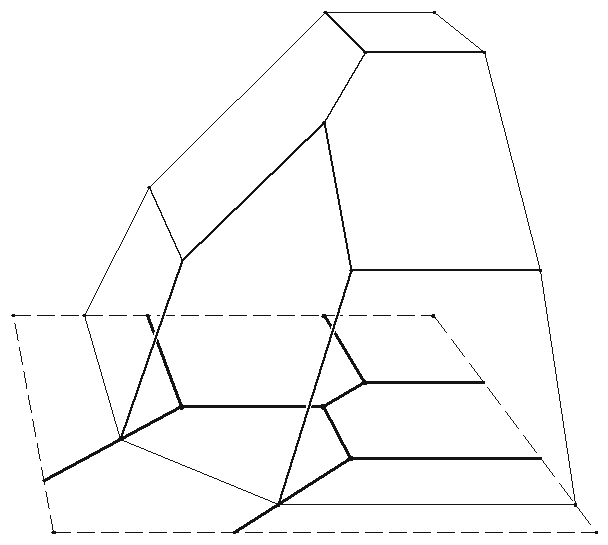
\includegraphics[width=0.4\textwidth]{Pics/conica.png}
				\\ \vspace{3pt}
				\emph{Rappresentazione di una conica tropicale}
				\vspace{6pt}
			\end{center}
			
			In generale è possibile anche tropicalizzare una qualsiasi varietà algebrica: la cosa fondamentale è che, tropicalizzando, si ottiene un oggetto geometrico più semplice, una sorta di \emph{poliedro} con alcune facce infinite, detto \emph{complesso poliedrale}, nelle cui proprietà si leggono molte delle proprietà della varietà algebrica di partenza come, per esempio, la dimensione, cioè il numero dei parametri indipendenti da cui dipendono i suoi punti.
			
			Consideriamo un modello probabilistico di evoluzione del DNA che sia algebrico, nel senso che i vincoli posti sulle possibili distribuzioni di probabilità siano dati da polinomi (gli invarianti filogenetici): questi polinomi descrivono una varietà algebrica $V$ che chiameremo varietà algebrica del modello probabilistico. Tropicalizzando $V$ si ottengono algoritmi per valutare in maniera efficiente le probabilità delle osservazioni, utili per applicare il principio di massima verosimiglianza nella ricerca delle filogenie.
			
			Tutte queste idee matematiche, pur avendo la loro radice in metodi piuttosto standard della geometria algebrica, sono state sviluppate solo di recente per raccogliere le sfide della filogenetica. In particolare, la matematica tropicale pone a suo fondamento un processo di semplificazione drastica dei dati di un problema complesso: un processo caratteristico delle esigenze della biologia teorica. La matematica tropicale non sarà forse lo strumento decisivo per la biologia, ma di certo giocherà un ruolo importante per lo sviluppo delle scienze naturali e della matematica stessa.
			\end{subsubsection}
		\end{subsection}
	
	\end{section}
\end{document}